\documentclass{report}
\usepackage[a4paper]{geometry}
\usepackage{graphicx}
\usepackage{hyperref}
\usepackage{float}
\usepackage{tikz}
\usepackage{amsmath}
\usepackage[affil-it]{authblk}\hypersetup{
    colorlinks,
    citecolor=black,
    filecolor=black,
    linkcolor=black,
    urlcolor=black
}
\usepackage{apacite}
\usepackage[authoryear]{natbib}

\title{Evolutionary Models with a Large Number of Genes}
\author{
    Mher Saribekyan, Suren Hakobyan, Davit Badalyan\\
    Instructor: Varazdat Stepanyan 
}
\affil{American University of Armenia}
\date{November 2024}
\begin{document}
\maketitle
\tableofcontents
\section{Abstract}
\section{Methods}
\subsubsection{Creature}
A creature is defined with its genome, position and energy.
The genome consists of 5 genes that represent certain characteristics of that creature.
The position shows the creature's position in the grid and the energy shows its energy level.
\subsubsection{Food}
Food are randomly generated when a simulation is initiated and randomly spawns in each timestep, but with a predefined limit.
\subsubsection{Energy}
A creature starts with predefined base energy level, and dies when the energy level reaches 0.
The creatures gains energy by consuming food or winning an attack against another creature, and loses energy when moving.
\subsubsection{Attack}
A creature has a gene for its level of aggression, which shows how likely it is to initiate an attack.
The winner is determined by the strength gene. The winner gains energy, while the loser dies.
\subsubsection{Reproduction and Mutations}
If a creature gains energy with a certain ratio of its maxmimum energy, it reproduces and gives 1 offspring, and loses a certain ratio of its energy.
The offspring is spawned in an adjacent positon and each gene is copied from its parent, with a certain probability for each gene to change by a value of 1.
\subsection{Memory optimization}
The creature is defined as an unsigned 32-bit integer, where the first 16 bits represent the genome, the next 12 bits represent its position cell and the last 4 bits represent the energy.
\begin{table}[H]
\begin{center}
    \begin{tabular}{|p{0.11\linewidth} |p{0.08\linewidth}|p{0.7\linewidth}|}
    \hline
    Gene & Bits & Description  \\\hline
    Speed & 2 & Takes values between 1 and 4, showing the Manhattan distance the creature can walk in a single timestep.\\\hline
    Eyesight & 3 & Takes values between 0 and 7, showing the Manhattan distance the creature can see.\\\hline
    Aggression & 3 & Takes values between 0 to 7, mapped to 0\% - 100\%, showing the probability of the creature attacking another creature in the same cell. \\\hline
    Strength & 4 & Takes values between 1 and 16, which determines the winner in a fight \\\hline
    Stamina & 4 & Takes values between -7 and 8, which is added to the base energy level, when generating the creature\\\hline
\end{tabular}
\caption{Creature characteristics and their descriptions}
\end{center}
\end{table}
\begin{figure}[!h]
\begin{center}
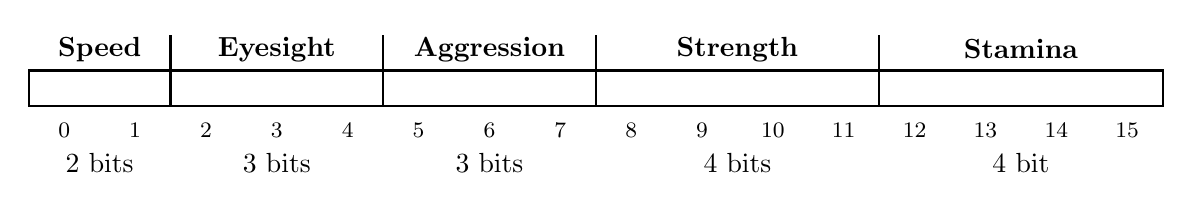
\begin{tikzpicture}[scale=0.9]
    % Draw the main rectangle for the 32 bits
    \draw[thick] (-0.5, 0) rectangle (15.5, 0.5);
    
    % Draw internal divisions for fields
    \foreach \x in {1.5, 4.5, 7.5, 11.5} {
        \draw[thick] (\x, 0) -- (\x, 1);
    }

    % Label the fields
    \node at (0.5, 0.8) {\textbf{Speed}};
    \node at (3, 0.8) {\textbf{Eyesight}};
    \node at (6, 0.8) {\textbf{Aggression}};
    \node at (9.5, 0.8) {\textbf{Strength}};
    \node at (13.5, 0.8) {\textbf{Stamina}};
    
    % Add labels for the bit positions (0-31)
    \foreach \x in {0, 1, ..., 15} {
        \node[anchor=north] at (\x, -0.1) {\footnotesize \x};
    }

    % Field descriptions under each field
    \node at (0.5, -0.8) {2 bits};
    \node at (3, -0.8) {3 bits};
    \node at (6, -0.8) {3 bits};
    \node at (9.5, -0.8) {4 bits};
    \node at (13.5, -0.8) {4 bit};
\end{tikzpicture}
\caption{Gene storage}
\end{center}
\end{figure}
\begin{figure}[!h]
\begin{center}
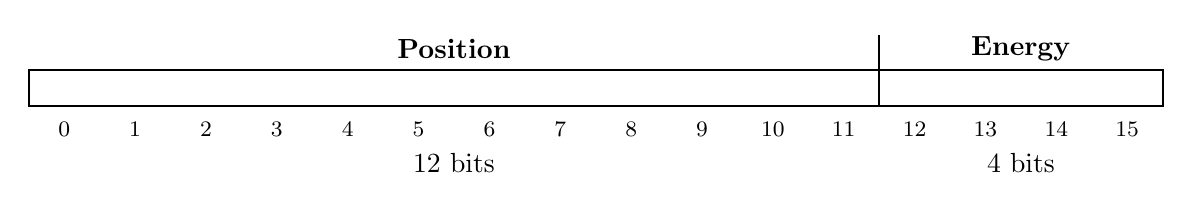
\begin{tikzpicture}[scale=0.9]
    % Draw the main rectangle for the 32 bits
    \draw[thick] (-0.5, 0) rectangle (15.5, 0.5);
    
    % Label the fields
    \node at (5.5, 0.8) {\textbf{Position}};
    \draw[thick] (11.5, 0) -- (11.5, 1);
    \node at (13.5, 0.8) {\textbf{Energy}};
    
    % Add labels for the bit positions (0-31)
    \foreach \x in {0, 1, ..., 15} {
        \node[anchor=north] at (\x, -0.1) {\footnotesize \x};
    }

    % Field descriptions under each field
    \node at (5.5, -0.8) {12 bits};
    \node at (13.5, -0.8) {4 bits};
\end{tikzpicture}
\caption{Position storage}
\end{center}
\end{figure}
The creatures are stored in a list and are iterated over in every timestep.
\section{Results}
The following constants were chosen for our simulations:
\begin{table}[H]
    \begin{center}
        \begin{tabular}{|p{0.24\linewidth} |p{0.08\linewidth}|p{0.55\linewidth}|}
        \hline
        Constant & Value & Notes  \\\hline
        Grid size & \(64\) & \(2^6\times 2^6\) grid\\\hline        
        Food cap & 0.05 & 5\% of the grid\\\hline
        Init creatures & 0.01 & We start with 1\% of the grid being creatures\\\hline
        Steps & 10000 & Number of timesteps\\\hline
        Base energy & 8 & Base energy\\\hline
        Energy from food & 5 & Energy gained from consuming food\\\hline
        Energy from creature & 8 & Energy gained from consuming another creature\\\hline
        Energy ratio to reproduce & 0.9 & When energy level reaches 90\% of the creatures max energy, it reproduces\\\hline
        Energy ratio for reproduce & 0.2 & 20\% of energy is consumed for reproduction\\\hline
        Number of children & 1 & Each reproduction only produces a single offspring\\\hline
        Mutation probability & 0.01 & There is a 1\% change for each gene to mutate during reproduction\\\hline
    \end{tabular}
    \caption{Creature characteristics and their descriptions}
    \end{center}
    \end{table}
\section{Discussion}
\nocite{*}
\bibliographystyle{apacite}
\bibliography{refs}
\end{document}
